Die Tschebyscheff-Polynome $T_n(x)$ für $n\in\mathbb{N}$ sind durch
die Beziehung \[
T_n(\cos z) = \cos nz
\]
definiert.
\begin{teilaufgaben}
\item
Verwenden Sie die Substitution $x=\cos z$, um das Skalarprodukt
\[
\langle f(x),g(x)\rangle
=
\int_{-1}^1 f(x)g(x) \frac{dx}{\sqrt{1-x^2}}
\]
von Funktionen auf dem Intervall$[-1,1]$
als Integral über das Intervall $[0,\pi]$ auszudrücken.
\item
Rechnen Sie direkt nach, dass die Tschebyscheff-Polynome bezüglich des
Skalarproduktes
\(
\langle \;\,,\;\rangle
\)
orthogonal sind.
\item
Berechnen Sie die Norm $\|T_n\|$ der Tschebyscheff-Polynome.
Beachten Sie insbesondere den Spezialfall $n=0$.
\item
Schreiben Sie die Funktion $f(x)$ als Reihe von Tschebyscheff-Polynomen.
\end{teilaufgaben}

\begin{loesung}
\begin{teilaufgaben}
\item
Wir berechnen die Skalarprodukte mit der Substitution $x=\cos z$
mit $dx = -\sin z \,dz$.
Das Skalarprodukt der Funktionen $f$ und $g$ wird dann zu
\begin{equation}
\langle f,g\rangle
=
\int_\pi^0 f(\cos z) g(\cos z) \frac{-\sin z \,dz}{\sqrt{1-\cos^2z}}
=
\int_0^\pi f(\cos z) g(\cos z) \,dz.
\label{buch:201:eqn:skalarprodukt}
\end{equation}
\item
Mit der Formel \eqref{buch:201:eqn:skalarprodukt} für das
Skalarprodukt finden wir für $n\ne m$
\begin{align*}
\langle T_n,T_m\rangle
&=
\int_0^\pi T_n(\cos z)T_m(\cos z)\,dz
=
\int_0^\pi \cos nz \cos mz\,dz
\\
&=
\frac12 \int_0^\pi \cos(n-m)z +\cos (n+m)z\,dz
\\
&=
\frac12\biggl[\frac{\sin(n-m)z}{n-m} + \frac{\sin(n+m)z}{n+m}\biggr]_0^\pi
=
\frac12\biggl(\frac{\sin(n-m)\pi}{n-m} + \frac{\sin(n+m)\pi}{n+m}\biggr).
\end{align*}
Da $n-m$ und $n+m$ ganzzahlig sind, sind $(n-m)\pi$ und $(n+m)\pi$
Nullstellen der Sinusfunktion und es folgt $\langle T_n,T_m\rangle = 0$.
\item
Die Norm von $T_n$ ist das Skalarprodukt von $T_n$ mit sich selbst,
also wieder mit Formel \eqref{buch:201:eqn:skalarprodukt} für $n\ne 0$
\begin{align*}
\|T_n\|^2
&=
\int_0^\pi T_n(\cos z)^2\,dz
=
\int_0^\pi \bigl( \cos nz\bigr)^2\,dz
=
\int_0^\pi \frac12\bigl(1 + \cos 2nz\bigr)\,dz
\\
&=
\frac{\pi}{2} + \int_0^\pi \cos 2nz\,dz
=
\frac{\pi}{2} + \biggl[\frac{\sin 2nz}{2n}\biggr]_0^\pi.
\end{align*}
Der zweite Term verschwindet wie in Teilaufgabe a) und es folgt
$\|T_n\|=\sqrt{2/\pi}$.

Für $n=0$ ist
\[
\|T_0\|^2
=
\int_{0}^\pi T_0(\cos z)^2\,dz
=
\int_{0}^\pi \,dz
=
\pi,
\]
also $\|T_0\|=\sqrt{\pi}$.
\item
Die in Teilaufgabe c) berechnete Norm ermöglicht jetzt, die orthonormierte
Funktionenfamilie
\begin{align*}
t_n(x) &= \sqrt{\frac{2}{\pi}} T_n(x)\qquad n>0\\
t_0(x) &= \sqrt{\frac{1}{\pi}} T_0(x)
\end{align*}
zu definieren.
Mit diesen Funktionen lässt sich jede Funktion auf dem Intervall $[-1,1]$
als Reihe
\begin{align*}
f(x)
&=
\sum_{n=0}^\infty
\langle t_n,f\rangle \cdot t_n(x)
=
\frac{1}{\pi}
\biggl\langle \sqrt{\frac{1}{\pi}} T_0,f\biggr\rangle
+
\sum_{n=1}^\infty
\biggl\langle \sqrt{\frac{2}{\pi}} T_n,f\biggr\rangle
\cdot
\sqrt{\frac{2}{\pi}}
T_n(x)
\\
&=
\frac{1}{\pi}
\langle T_0,f\rangle
+
\frac{2}{\pi}
\sum_{n=1}^\infty
\langle T_n,f\rangle \cdot T_n(x)
\end{align*}
schreiben.
Bei der Berechnung der Skalarprodukte tritt $\sqrt{1-x^2}$ als Nenner
auf, der Nullstellen an den Intervallenden hat.
Mit der Formel~\eqref{buch:201:eqn:skalarprodukt} kann man diese 
Schwierigkeit vermeiden und erhält die Formel
\[
\langle T_n,f\rangle
=
\int_0^\pi \cos nz \cdot f(\cos z)\,dz.
\]
Die Reihe ist daher
\[
f(x)
=
\frac{1}{\pi}
\int_0^\pi f(\cos z)\,dz
+
\frac{2}{\pi}
\sum_{n=1}^\infty
\biggl(
\int_0^\pi f(\cos z)\cos nz \,dz
\biggr)
\cdot
T_n(x).
\qedhere
\]
\end{teilaufgaben}
\end{loesung}

\begin{figure}
\centering
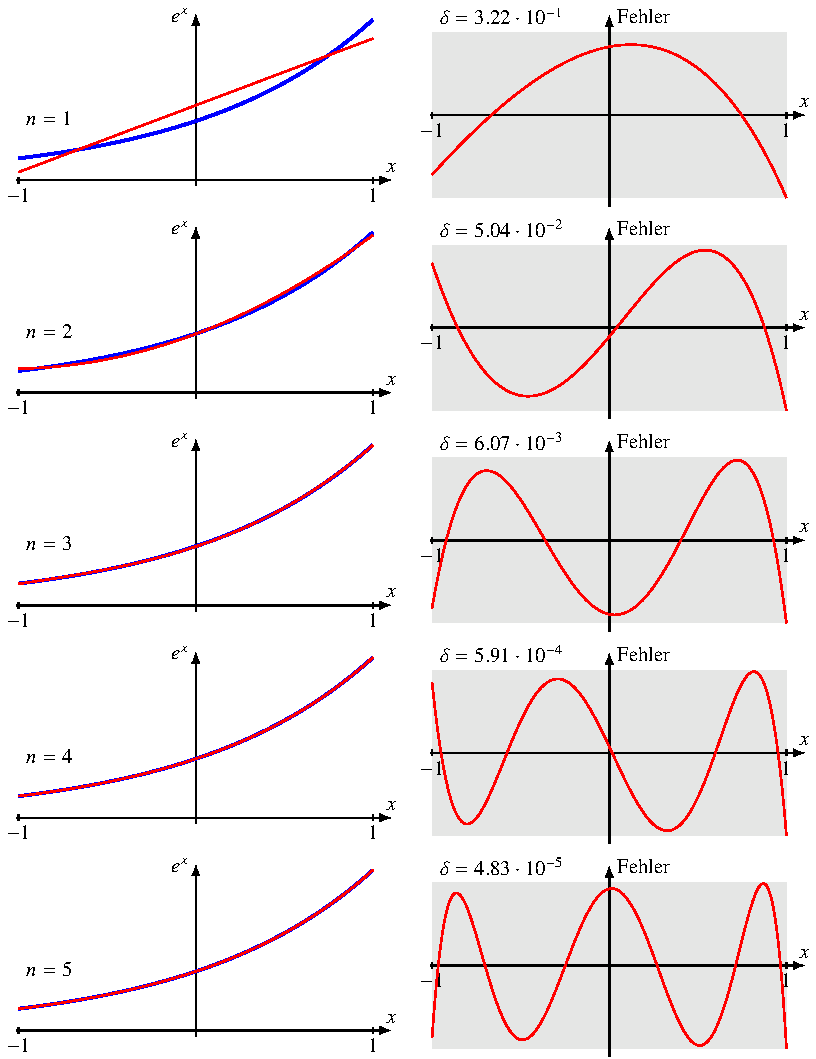
\includegraphics{chapters/020-orthofkt/images/chebexp.pdf}
\caption{Approximation der Exponentialfunktion im Intervall
$[-1,1]$ durch eine Reihe von Tschebyscheff-Polynomen
\label{buch:201:fig:exp}}
\end{figure}
\begin{figure}
\centering
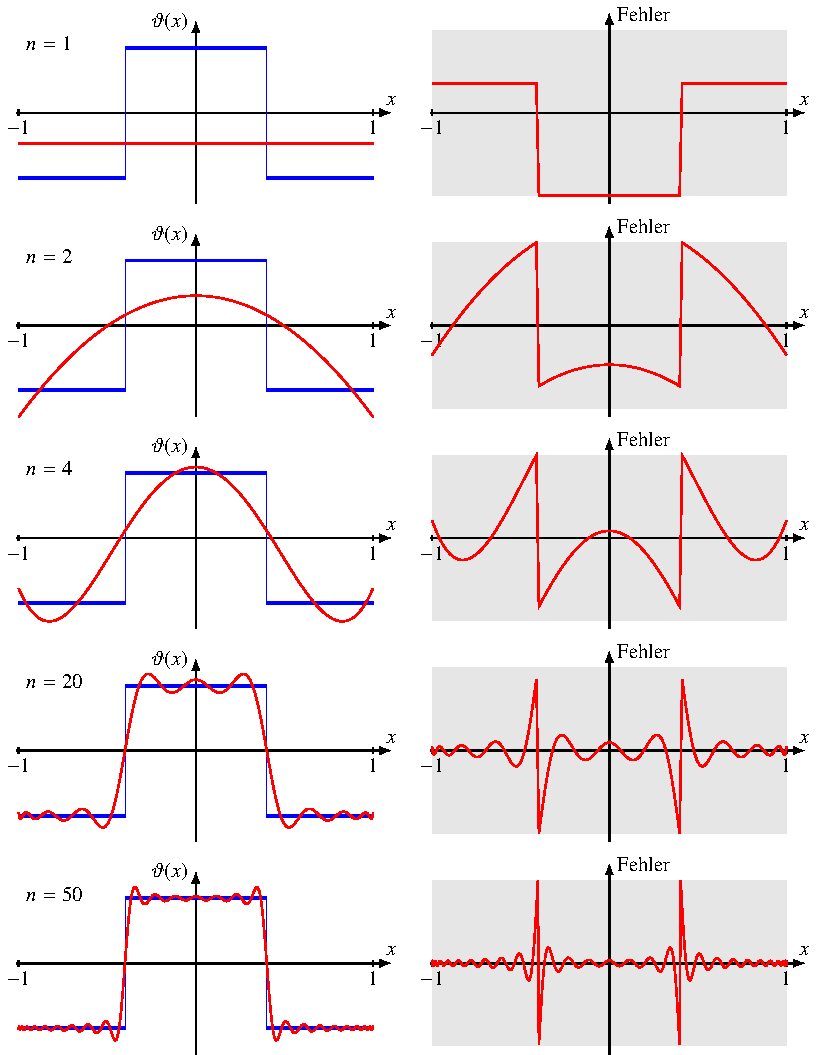
\includegraphics{chapters/020-orthofkt/images/chebrect.pdf}
\caption{Approximation einer Rechteckfunktion im Intervall
$[-1,1]$ durch eine Reihe von Tschebyscheff-Polynomen.
Wie bei der Fourier-Transformation ist das sogenannte {\em Gibbs-Phänomen}
\index{Gibbs-Phänomen}%
an den Sprungstellen beobachtbar.
\label{buch:201:fig:rect}}
\end{figure}

Die Aufgabe zeigt eine Möglichkeit, stetige Funktionen auf dem Intervall
$[-1,1]$ gleichmässig durch Polynome zu approximieren.
In den Abbildungen~\ref{buch:201:fig:exp} und \ref{buch:201:fig:rect}
sind die Exponentialfunktion bzw.~ein Rechteckfunktion auf diese
Weise approximiert.
Abbildung~\ref{buch:201:fig:exp} zeigt die rasche Konvergenz
der Reihe,
Abbildung~\ref{buch:201:fig:rect} das Gibbs-Phänomen an den
Sprungstellen.



